
\begin{figure*}[ht!]
  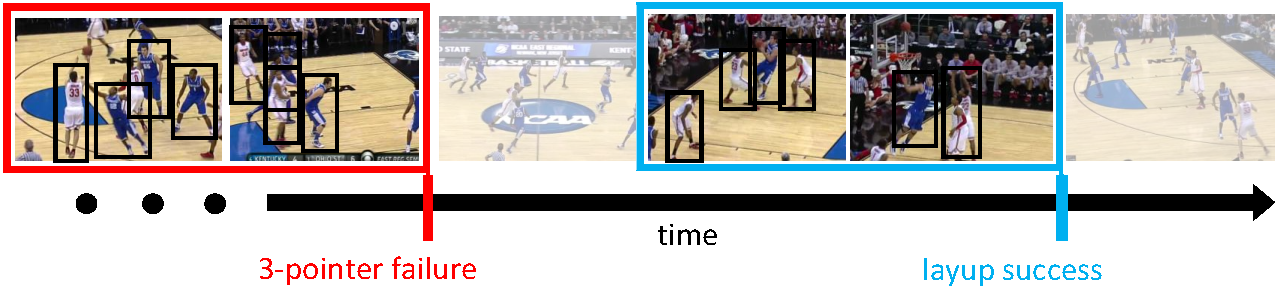
\includegraphics[width=6.5 in]{images/dataset_figure_cropped.pdf}
  \caption{Our dataset contains timestamp annotations for 11 basketball events
    in long untrimmed videos. Additionally, we also provide bounding boxes for player
    detections obtained from a multibox model trained on a subset of training
  video frames.}
\end{figure*}



\section{Related Work}


\noindent \textbf{Action recognition datasets}
Various datasets have been proposed for action recognition,
including KTH \cite{KTH}, HMDB \cite{HMDB}
UCF101 \cite{UCF101}, TRECVID-MED \cite{MED11} and Sports-1M \cite{Karpathy_CVPR14}.
More recently, THUMOS \cite{THUMOS} and ActivityNet \cite{ActivityNet} also provide a detection
setting with temporal annotations for the location of the action in a temporally untrimmed video.
There are also fine-grained datasets
in specific domains such as MPII cooking \cite{Finegrained_cooking} and breakfast \cite{Breakfast}.
However, most of these dataset focus on single-person activities with little
need to recognize the people responsible for the event. On the other
hand, publicly available multi-person activity datasets 
such as \cite{Choi_ICCV09,Ryoo_10} are restricted
to a very small number of videos.  One of the contributions of our work is 
a multi-player basketball dataset with dense temporal event annotations in
long videos, which we discuss in Section~\ref{sec:data}.

\noindent \textbf{Action recognition in videos}
Traditionally, well engineered features have proved quite effective for video
classification and retrieval tasks
\cite{Dalal_ECCV06,Jain_CVPR13,Jiang_ECCV12,Laptev_CVPR08,
Niebels_ECCV10,Oh_MVA14,Oneata_ICCV13,Peng_ECCV14,Sadanand_CVPR12,Wang_BMVC09,Wang_CVPR11}.
The improved dense trajectory (IDT) features \cite{Wang_CVPR11} achieve
competetive results on standard video datasets.  In the last few years,
end-to-end trained deep network models
\cite{Ji_PAMI13,Karpathy_CVPR14,Simonyan_2014,Tran_arxiv14} were shown to be comparable and
at times better than these features for various video tasks.  Other works like
\cite{Xu_2015,Zha_2015,Wang_arxiv15} explore methods for pooling such
features for better performance.

Recent works using Recurrent Neural Networks (RNN) have achieved
state-of-the-art results for both event recognition and caption-generation
tasks \cite{Donahue_arxiv14,Ng_arxiv15,Srivastava_2015,Yao_arxiv15}.
We follow this line of work with addition of attention mechanism
to attend to the event participants.

\noindent \textbf{Muti-person video analysis}
Activigy recognition models for events with well defined group structures such
as parades have been presented in
\cite{Vaswani_CVPR03,Intille_CVIU01,Moore_AAAI02,Khan_ACM05}.  They utilize the
structured layout of participants to identify group events. More
recently, \cite{Lan_PAMI12,Choi_ICCV09,Khodabandeh_arxiv15} use context as a
cue for recognizing interaction based group activities.  While the models
multi-person events, these methods are restricted to smaller
datasets such as UT-Interaction\cite{Ryoo_10}, Collective activity
\cite{Choi_ICCV09} and Nursing home\cite{Lan_PAMI12}.

\noindent \textbf{Attention models}
Itti et al. \cite{Itti_PAMI98} explored the idea of saliency based attention in
images, with other works like \cite{Shapovalova_NIPS13} using eye-gaze data as
a means for learning attention.
Other approaches such as Gkioxari et al. \cite{Gkioxari_arxiv14} and Raptis et al. \cite{Raptis_CVPR12}
automatically localize a spatio-temporal tube in the video corresponding to the action.
Another similar work\cite{Gkioxari_ICCV15} localize boxes in static images
for action recognition.

Recently, \cite{Bahdnau_arxiv14} showed that
attention based RNN models can effectively align input words in a sentence to
output words for machine translation.  Following this work, attention was used
for aligning regions in an image to output words for image-captioning
\cite{Xu_arxiv15} and frames in a video with output words for video-captioning
\cite{Yao_arxiv15}.  In all these methods, attention aligns a sequence of input
features with words of an output sentence. However, in our work we use
attention to identify the most releavant person to the overall event during
different phases of the event.  Further, in our setting the attended set of
player detections changes between frames. This leads to interesting
model choices, which we will discuss in Section~\ref{sec:methods}.

\noindent \textbf{Action recognition datasets}
Action recognition in videos has eveolved with the introduction of more
sophisticated datasets starting from smaller KTH \cite{KTH}, HMDB \cite{HMDB}
to larger , UCF101 \cite{UCF101}, TRECVID-MED \cite{MED11} and Sports-1M \cite{Karpathy_CVPR14}
datasets.
More recently, THUMOS \cite{THUMOS} and ActivityNet \cite{ActivityNet} also provide a detection
setting with temporal annotations for actions in untrimmed videos.
There are also fine-grained datasets
in specific domains such as MPII cooking \cite{Finegrained_cooking} and breakfast \cite{Breakfast}.
However, most of these dataset focus on single-person activities with hardly
any need for recognizing the people responsible for the event. On the other
hand, publicly available multi-person activity datasets \cite{Choi_ICCV09,Ryoo_10,VIRAT} are restricted
to a very small number of videos.  One of the contributions of our work is 
a multi-player basketball dataset with dense temporal event annotations in
long videos. We provide more details in the next section.

\noindent \textbf{Person detection and tracking}. There is a very
large literature on person detection and tracking. Here we just
mention a few key papers.
For person detection, we use the CNN-based multibox detector from
\cite{Szegedy13}.
For person tracking, we use the KLT tracker from
\cite{Veenman_PAMI2001}.
There is also work on player identification (e.g., \cite{Lu2013}), but
in this work, we do not attempt to distinguish individual players.
